\documentclass{article}
\usepackage[left=2cm, right=2cm, top=0cm]{geometry}
\usepackage{amsmath}
\usepackage{amssymb}
\usepackage{graphicx}
\usepackage{tikz}
\usepackage{comment}
\usepackage{enumitem}
\usepackage{float}
\usepackage{hyperref}
\usepackage[margin=2cm]{caption}
\setlength\parindent{0pt}
\hypersetup{
    colorlinks,
    citecolor=green,
    filecolor=black,
    linkcolor=blue,
    urlcolor=blue
}

\begin{document}
\title{Assignment 2: Constrained Optimization and the KKT Conditions}
\author{Jacob Puthipiroj}
%\date{}
\maketitle

\section*{KKT Conditions for Linear Programming}


A linear program can be expressed in canonical form as:
$$ \min_x c^Tx \qquad \text{subject to} \qquad Ax \leq b$$
for matrices $A \in \mathbb{R}^{m \times n}, b \in \mathbb{R}^{m \times 1}$ and $c \in \mathbb{R}^{n \times 1}$.

The Lagrangian would be $$ \mathcal{L}(x,\lambda) = c^Tx - \lambda(Ax-b) $$
In this case, $\lambda$ is a vector of $n$ values. 
Primal feasibility, dual feasibility, complementary slackness, and lagrange stationarity

\section*{Expressing $l_1$ and $l_\infty$ Regression Problems as Linear Programs}
Specifically, by defining slack variables and inequality constraints as needed.


\section*{Solving $l_1$ and $l_\infty $ regression problems using CVXPY}

\begin{figure*}[h]
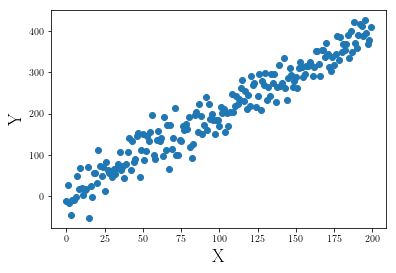
\includegraphics[scale = 0.6]{Line Graph.png}
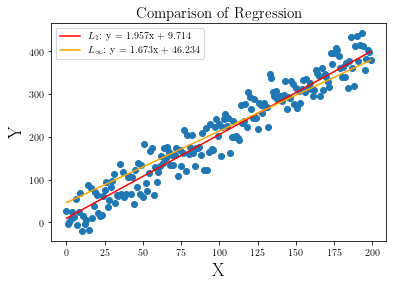
\includegraphics[scale = 0.6]{Comparison.png}
\caption{The contour plots, as well as the 3D projection plot indicates that there is a unique maximum over the domain. This is critical point is approximately $x^* \approx [1 \textrm{m},1 \ \textrm{rad} ]$.}
\end{figure*}




\end{document}